\begin{titlepage}
\begin{center}

% Upper part of the page. The '~' is needed because only works if a paragraph has started.
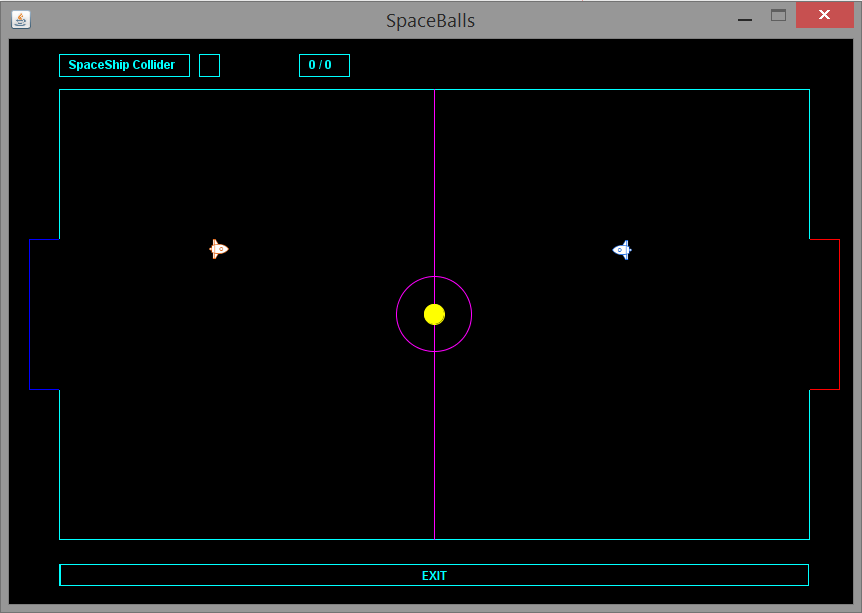
\includegraphics[width=15cm]{./TerrainAvecJoueur.png}~\\[1cm]

\textsc{\LARGE Langage avancé de programmation}\\[1.5cm]

\textsc{\Large }\\[0.5cm]

% Title
\HRule \\[0.4cm]

{\huge \bfseries Projet Java\\
GénialBall \\[0.4cm] }

\HRule \\[1.5cm]

% Author and supervisor
\begin{minipage}{0.4\textwidth}
\begin{flushleft} \large
\emph{Auteur:}\\
Nicolas Sias 2TL1\\
Youri Mouton 2TL2
\end{flushleft}
\end{minipage}
\begin{minipage}{0.4\textwidth}
\begin{flushright} \large
\emph{Année académique:} \\
2014-2015
\end{flushright}
\end{minipage}

\vfill

\end{center}
\end{titlepage}